\chapter{Analyse des données}


\section{Data Mining - Analyse exploratoire}

\subsection{Pre-processing}
%Description du dataset (rapidement, le reste dans un codebook)\\

%Mise en forme du dataset, une sortie à la fois vs plusieurs sorties etc \\
%On considère les données gustatives et les défauts physiques comme des sorties -> les prendre un par un ou tous ensemble\\

%Description du set, différentes parties des données, éventuelles données manquantes\\

Une grande partie de l'étape de préprocessing a été réalisée durant l'extraction des données. Il a en effet fallu extraire les données d'une manière uniforme et cohérente dès le départ afin de ne pas se retrouver avec des variables présentes uniquement dans certaines parties du set de données ou avec des variables incohérentes comme cela a été le cas de certains cafés qui avaient comme note de dégustation plus de cent points sur cent par exemple. Des éliminations ou des corrections ont été réalisées de manière automatisées ou manuelles afin de supprimer les erreurs. On notera parmi les corrections importantes le remplacement de virgules par des points, quelques erreurs de frappes (68.5 points sur 10 au lieu de 6.85 par exemple) ou encore des utilisations d'unités différentes. Le dataset résultant est décrit dans l'Annexe A de ce projet. Une fois cette étape de nettoyage réalisée, les premières informations ont pu être extraites des données.


\noindent Le schéma \ref{DatasetMaking} résume rapidement les différentes élimination d'observations au cours des étapes de construction du set de données. 

\begin{figure}[H]
	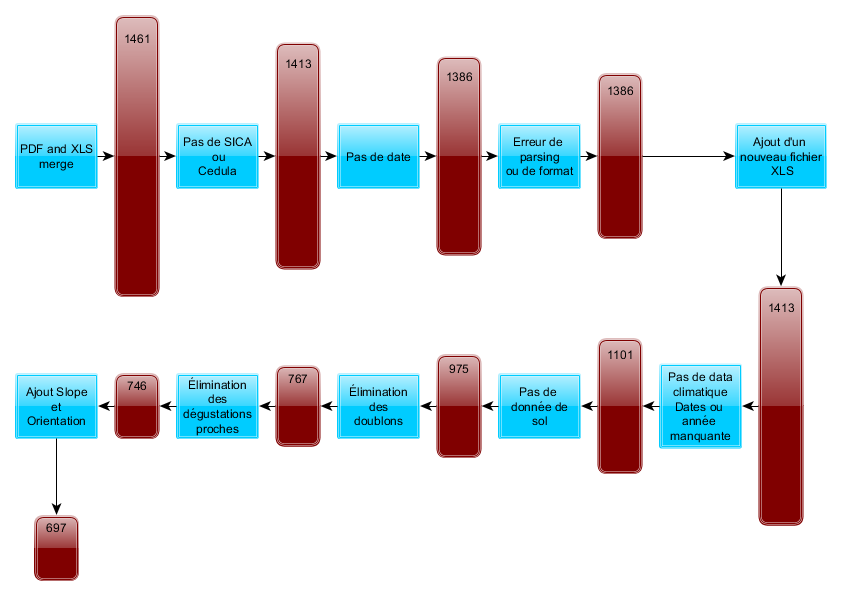
\includegraphics[scale=0.5]{Dataset_1}
	\caption{\label{DatasetMaking} Étape de construction du set de données et pertes d'observations.}
\end{figure}


%TODO Cases des observations - peuvent être recyclées après
\subsection{Emplacement des fermes}\label{EmpFermes} L'emplacement des différents cafés par rapport aux nombre de points est présenté sur la figure \ref{FincaVSPoints}. La catégorie 1 (non représentée) correspond aux cafés avec plus de 90 points, la 2 aux cafés avec plus de 85, la 3 aux cafés avec plus de 80 et la 4 aux cafés en dessous de 80, ne correspondant donc pas à la qualité "Specialty". On peut y voir que l'emplacement dans le département n'as pas d'incidence sur les résultats, la répartition des différentes classes étant très uniforme. 


\begin{figure}[H]
	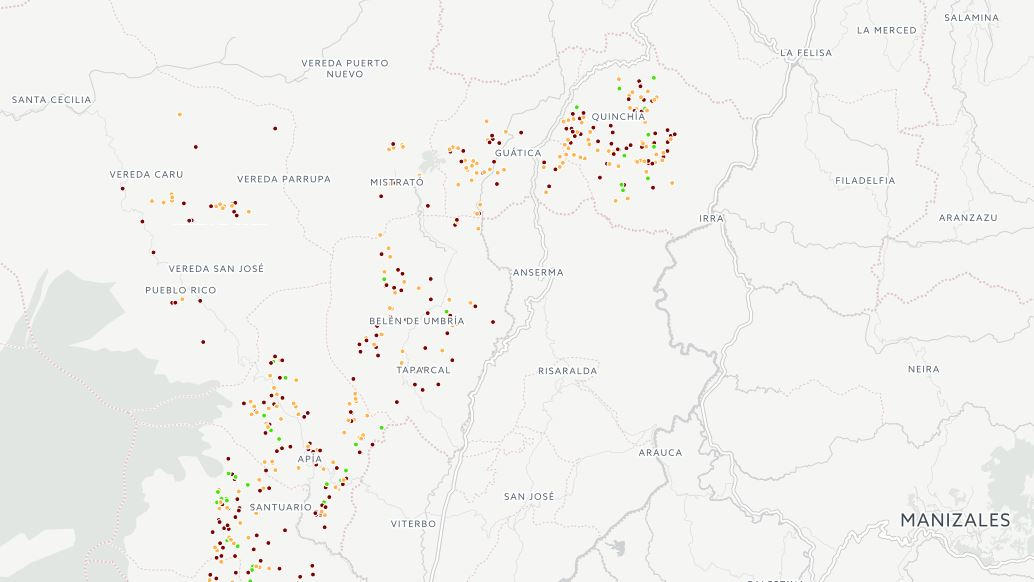
\includegraphics[scale=0.71]{Map_North}
	\newline
	\newline
	\newline
	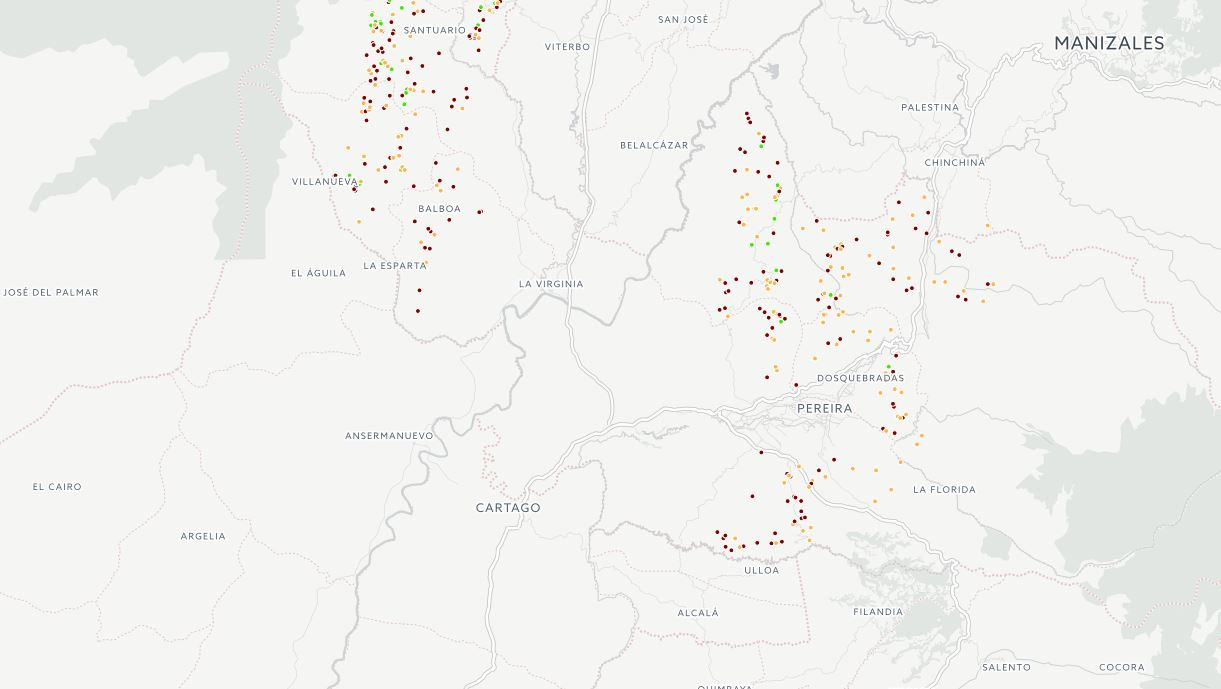
\includegraphics[scale=0.6]{Map_South}
	
	\begin{figure}[H]
		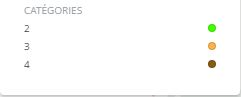
\includegraphics[scale=1]{Legend_Map2}
	\end{figure}
	\caption{\label{FincaVSPoints} Emplacement des fermes avec coloration selon le nombre de points attribués au café.}
\end{figure}


\subsection{Corrélations entre variables}

Afin d'avoir une bonne vue d'ensemble sur les variables et leurs liens, les matrices de corrélation ont été calculées pour toutes les variables. Premièrement la corrélation entre les différentes sorties. Sur la figure \ref{correlation_sorties1} on peut observer que les défauts physiques des grains ne sont que très peu liés entre eux ou avec les résultats de dégustation. On remarque cependant que les données gustatives du café sont fortement liées entre elles. 

\begin{figure}[H]
	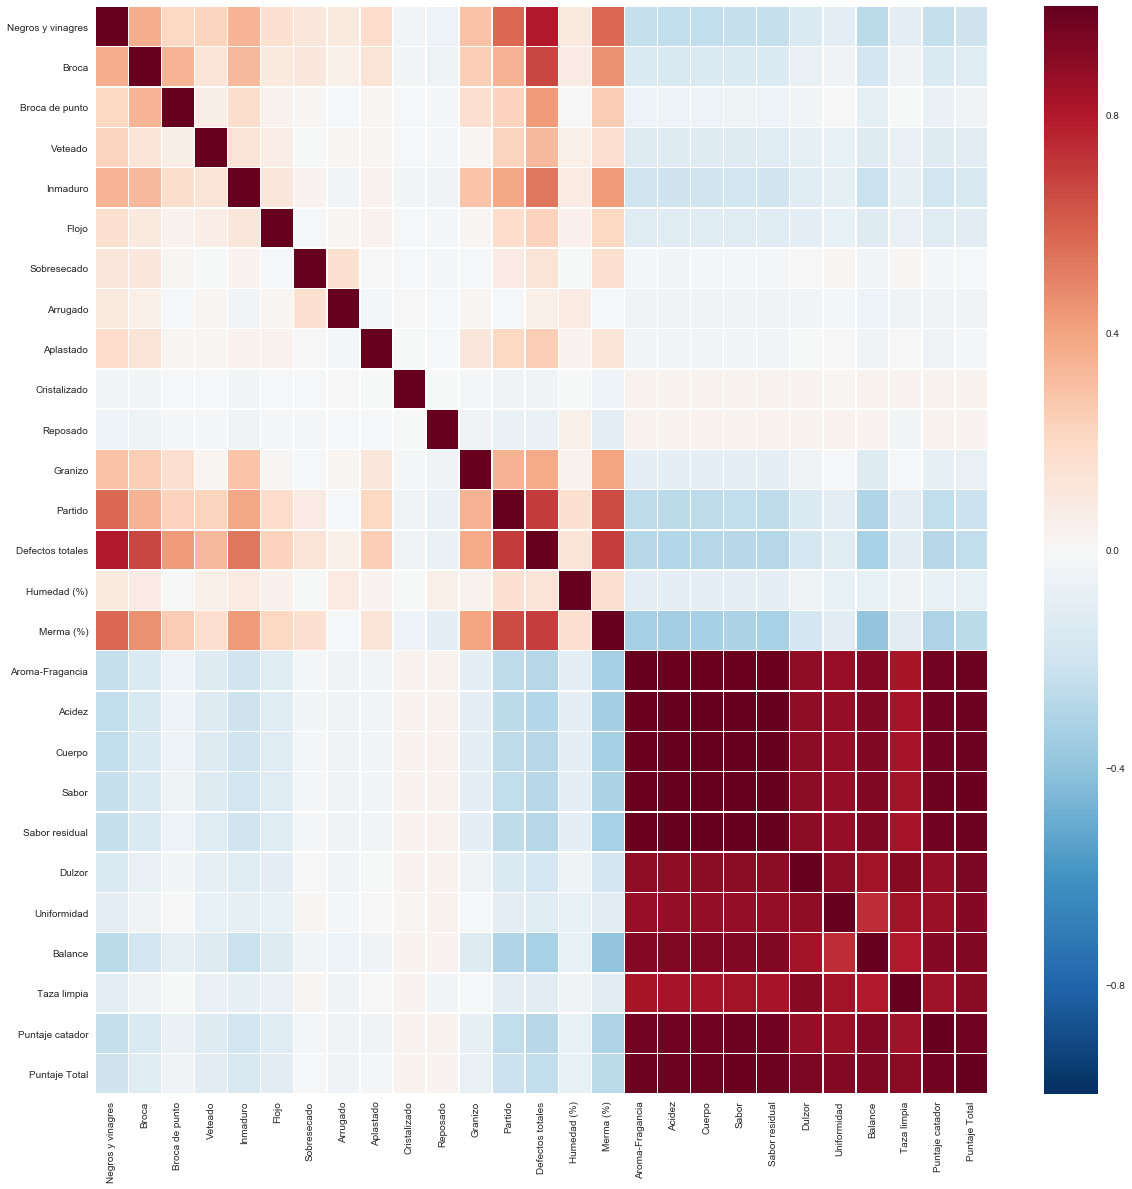
\includegraphics[scale=0.35]{correlation_sorties1}
	\caption{\label{correlation_sorties1} Matrice de corrélation entre les différentes sorties.}
\end{figure}


\noindent Sur la figure \ref{correlation_all1} on peut observer les corrélations entre toutes les variables. 


\begin{figure}[H]
	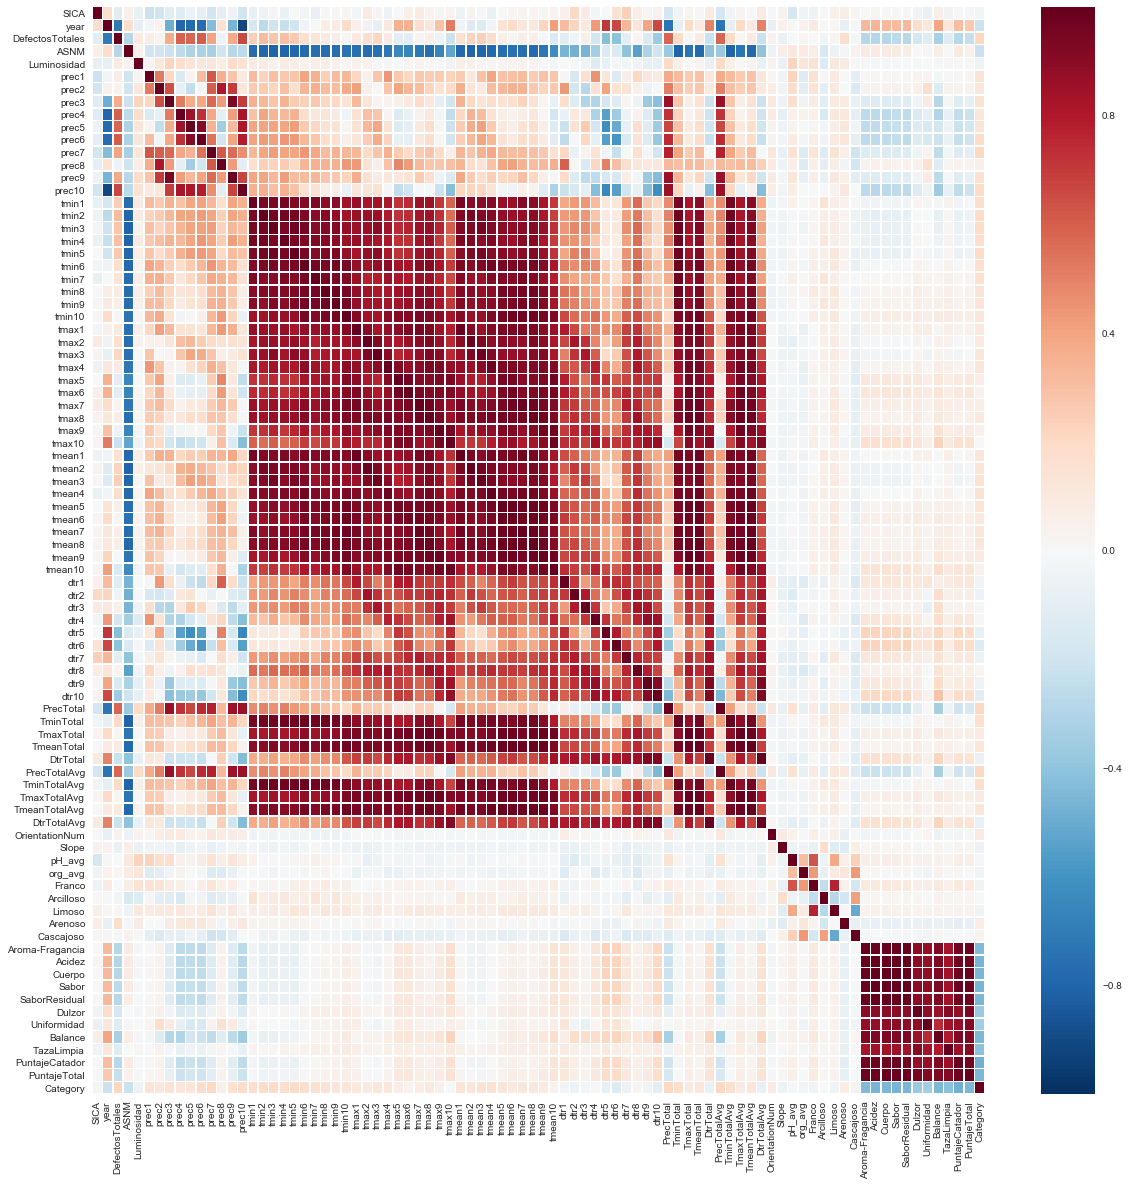
\includegraphics[scale=0.35]{correlation_all1}
	\caption{\label{correlation_all1} Matrice de corrélation entre toutes les variables.}
\end{figure}


\noindent On observe que les données de sol sont parfois corrélées entre-elles mais presque pas du tout avec les données climatiques. On peut donc déjà soulever que le climat n'a pas ou peu d'influence sur la texture, le pH ou le taux de matière organique du sol des zones étudiées. Les précipitations ont une influence importante sur les défauts physiques des grains, en revanche nous n'avons aucune variable qui a une corrélation marquée avec les points totaux et donc la qualité du café.   

%TODO garder un peu de place pour lorsqu'on ajoutera des données comme la pente, le soleil etc.


%TODO Parler des variétés de cafés et de quelques données les concernants (Moyennes de points, rendement par variété, altitude etc) 










\newpage
\subsection{Principal Component Analysis (PCA)}\label{PCAss}
La PCA, pour Analyse en Composantes Principales en français, est une méthode qui consiste à transformer un jeu de variables corrélées en nouvelles variables dé-corrélées les unes des autres. Ces nouvelles variables sont appelées composantes principales et permettent de rendre l'information moins redondante. Pour faire plus simple, l'utilité de la Composante Principale est de réduire le nombre de variables tout en gardant un maximum d'information. La figure \ref{PCAdefinition} montre une représentation graphique de la composante principale. 


\begin{figure}[H]
	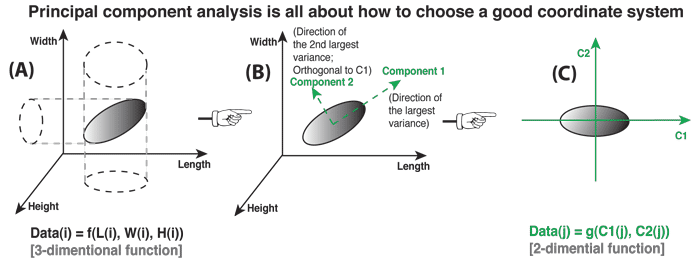
\includegraphics[scale=0.5]{PCA_1}
	\caption{\label{PCAdefinition} Description de l'Analyse en Composante Principale. (A) Description d'un objet simple de manière compliquée ( trois dimensions pour par exemple une ellipse en papier) (B) Trouver des nouvelles variables (axes de coordonnées) orthogonaux l'un à l'autre qui pointent dans les directions de la plus grande variance (C) Utiliser les nouvelles variables (axes) pour décrire l'objet d'une manière plus simple. }
\end{figure}

\paragraph{Résultats de la PCA}

L'analyse sur une version compacte des variables a donné les résultats présentés dans le tableau \ref{TablePCAResult1} et sur la figure \ref{FigurePCAResult1}. Une première analyse avait été effectuée sur le set de données complet, c'est-à-dire avec la totalité des données climatiques et non les moyennes, et les résultats se sont avérés similaires mais plus difficilement lisibles.  

\begin{table}[H]
	\centering
	
	\begin{tabular}{lllllll}
		Rotations       & PC1     & PC2     & PC3     & PC4     & PC5     & PC6     \\
		DefectosTotales & -0.0920 & -0.0994 & 0.1126  & -0.0904 & \textbf{0.5291}  & -0.0355 \\
		ASNM            & 0.0201  & \textbf{0.4183}  & 0.0638  & 0.0665  & -0.1267 & -0.0559 \\
		Luminosidad     & -0.0062 & -0.0178 & 0.2202  & -0.1228 & 0.1213  & -0.1294 \\
		PrecTotalAvg    & -0.0683 & -0.1792 & 0.1949  & -0.0507 & \textbf{0.5384}  & 0.1095  \\
		TminTotalAvg    & -0.0013 & \textbf{-0.4599} & -0.0001 & -0.1085 & 0.0528  & 0.0128  \\
		TmaxTotalAvg    & 0.0278  & \textbf{-0.4686} & -0.0531 & -0.0103 & -0.1613 & -0.0370 \\
		TmeanTotalAvg   & 0.0167  & \textbf{-0.4782} & -0.0330 & -0.0506 & -0.0786 & -0.0178 \\
		DtrTotalAvg     & 0.0555  & -0.3236 & -0.1028 & 0.1178  & -0.3796 & -0.0880 \\
		OrientationNum  & -0.0080 & -0.0032 & 0.0477  & -0.0241 & 0.0614  & \textbf{0.4606}  \\
		Slope           & 0.0071  & 0.0440  & -0.1277 & -0.0796 & -0.0342 & \textbf{0.4612}  \\
		pH Avg         & 0.0207  & 0.0149  & \textbf{0.4099}  & -0.3280 & -0.1111 & 0.1129  \\
		org Avg        & 0.0019  & 0.0427  & 0.2397  & -0.4616 & -0.1906 & -0.2169 \\
		Franco          & 0.0329  & -0.0271 & \textbf{0.5335}  & -0.0635 & -0.2088 & 0.1439  \\
		Arcilloso       & 0.0058  & -0.0156 & -0.2859 & -0.3538 & 0.0079  & 0.2955  \\
		Limoso          & 0.0190  & -0.0752 & \textbf{0.4779}  & \textbf{0.2327}  & -0.1418 & 0.2242  \\
		Arenoso         & -0.0303 & -0.0189 & 0.1254  & 0.0164  & 0.1284  & \textbf{-0.5509} \\
		Cascajoso       & -0.0051 & 0.0766  & -0.1646 & \textbf{-0.6555} & -0.0585 & -0.0839 \\
		Aroma.Fragancia & \textbf{0.3051}  & 0.0116  & -0.0013 & -0.0029 & 0.0028  & -0.0156 \\
		Acidez          & \textbf{0.3067}  & 0.0140  & -0.0010 & -0.0050 & 0.0003  & -0.0127 \\
		Cuerpo          & \textbf{0.3069}  & 0.0091  & 0.0012  & -0.0009 & 0.0053  & -0.0078 \\
		Sabor           & \textbf{0.3069}  & 0.0114  & 0.0026  & 0.0000  & 0.0168  & -0.0109 \\
		SaborResidual   & \textbf{0.3067}  & 0.0091  & 0.0009  & -0.0016 & 0.0093  & -0.0110 \\
		Dulzor          & \textbf{0.2887}  & -0.0178 & 0.0033  & -0.0012 & 0.1144  & 0.0120  \\
		Uniformidad     & \textbf{0.2794}  & -0.0051 & 0.0200  & 0.0050  & 0.1852  & 0.0340  \\
		Balance         & \textbf{0.2922}  & 0.0016  & -0.0203 & -0.0151 & -0.0908 & -0.0432 \\
		TazaLimpia      & \textbf{0.2749}  & -0.0172 & 0.0018  & -0.0133 & 0.1545  & 0.0004  \\
		PuntajeCatador  & \textbf{0.3033}  & 0.0116  & -0.0014 & -0.0096 & 0.0124  & -0.0006 \\
		PuntajeTotal    & \textbf{0.3089}  & 0.0009  & 0.0013  & -0.0047 & 0.0555  & -0.0037 \\
	\end{tabular}
\caption{\label{TablePCAResult1}Tableau des rotations des six premiers composants de la PCA avec mise en évidence des variables les plus importantes par composante.}
\end{table}


\begin{figure}[H]
	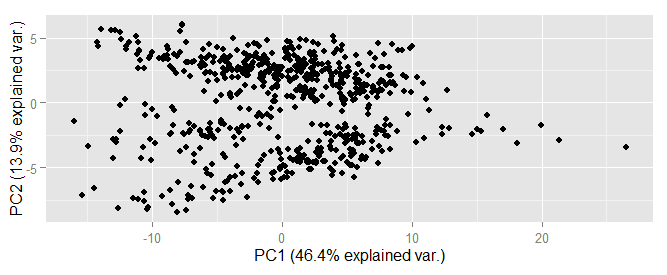
\includegraphics[scale=0.5]{PCA_AllVariables}
	\caption{\label{FigurePCAResult1} Résultats de la PCA sous forme graphique. }
\end{figure}


\paragraph{Première composante} La première composante met en évidence les 11 variables des points attribués au café ce qui suggère que ces variables ont tendance à varier ensemble. Cette tendance était déjà mise en évidence dans la matrice de corrélation au point \ref{correlation_sorties1}. 

\paragraph{Seconde composante} La seconde composante met en évidence les températures et l'altitude qui sont fortement liées. On peut donc voir ce composant comme décrivant à quel point le café est cultivé dans un lieu haut et froid. 

\paragraph{Troisième composante} La troisième composante met en évidence la texture limoneuse et franco du sol ainsi que le pH. Ce composant montre que les sols franco ont tendance à être plutot limoneux 

\paragraph{Quatrième composante} Met en évidence qu'un sol limoneux n'est pas rocailleux ce qui est logique mais pas important pour notre analyse.

\paragraph{Cinquième composante} Met en évidence que lorsque les précipitations augmentent, le pourcentage de grains déféctueux augmente lui aussi. Cette relation est visible sur la matrice de corrélation de la figure \ref{correlation_all1}. 

\paragraph{Sixième composante} Met en évidence le fait que la pente et l'orientation sont inversement corrélés à la quantité de sable dans le sol. Plus la pente est élevée, moins le sol sera sablonneux. 

% https://georgemdallas.wordpress.com/2013/10/30/principal-component-analysis-4-dummies-eigenvectors-eigenvalues-and-dimension-reduction/

%https://onlinecourses.science.psu.edu/stat505/node/54





\newpage
\subsection{Self-Organizing Map}
%TODO 

\subsubsection{U-Matrix}


\begin{figure}[H]
	\centering
	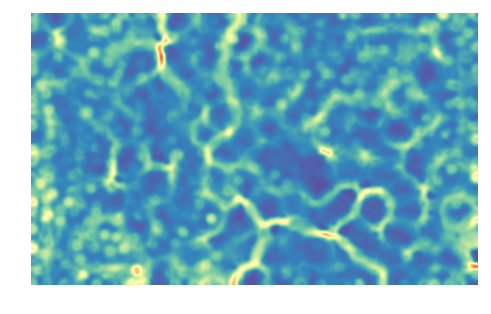
\includegraphics[width=0.7\linewidth]{SOM/SOM_Umatrix}
	\caption{U-Matrix de la carte SOM}
	\label{}
\end{figure}

\begin{figure}[H]
	\centering
	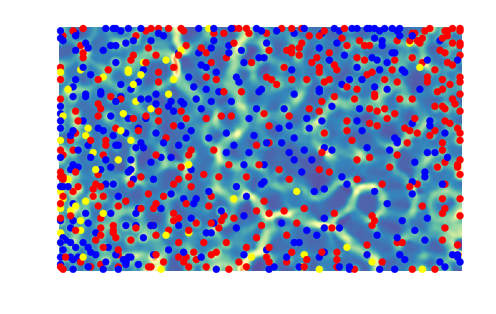
\includegraphics[width=1\linewidth]{SOM/SOM_Umatrix_Points_Category}
	\caption{U-Matrix avec les points. En jaune les cafés de catégorie 2,en bleu catégorie 3 et en rouge catégorie 4. Les catégories sont expliquées au point \ref{EmpFermes}}
	\label{}
\end{figure}

\subsubsection{Composants}



\begin{figure}[H]
	\caption{Composants de qualité - Variables de sortie}
	\centering
		\subfloat[Acidez]{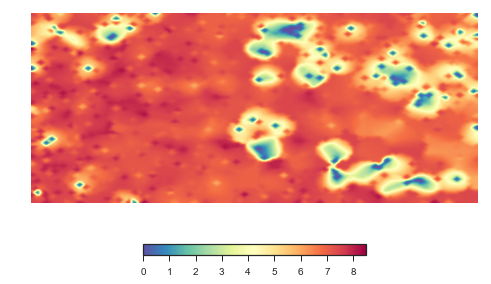
\includegraphics[width=.3\linewidth]{SOM/SOM_Acidez}}\hfill
		\subfloat[Aroma-Fragrancia]{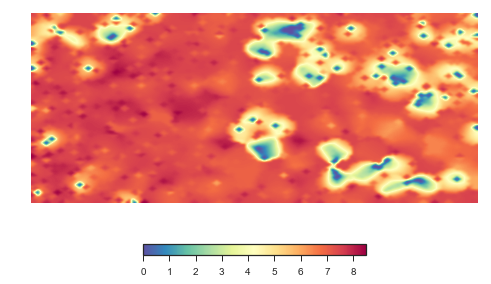
\includegraphics[width=.3\linewidth]{SOM/SOM_AromaFragrancia}}\hfill
		\subfloat[Cuerpo]{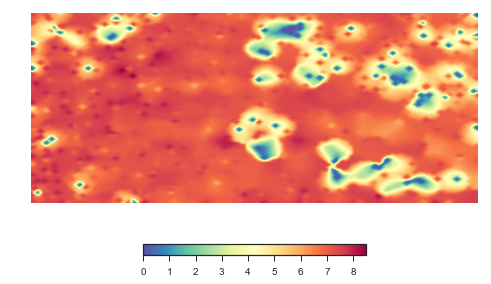
\includegraphics[width=.3\linewidth]{SOM/SOM_Cuerpo}}
		\newline
		\subfloat[Balance]{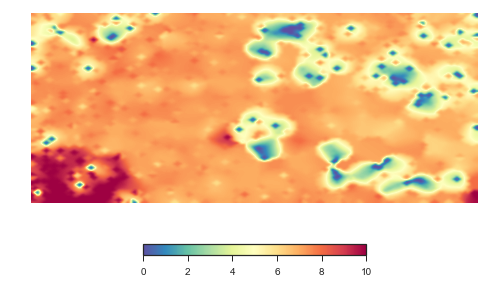
\includegraphics[width=.3\linewidth]{SOM/SOM_Balance}}\hfill
		\subfloat[Uniformidad]{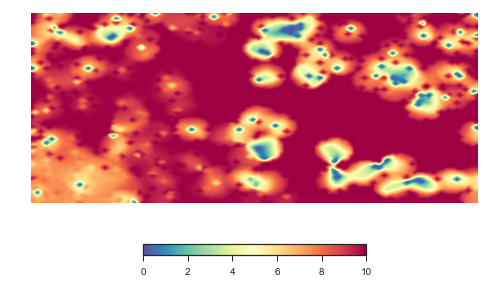
\includegraphics[width=.3\linewidth]{SOM/SOM_Uniformidad}}\hfill
		\subfloat[Taza Limpia]{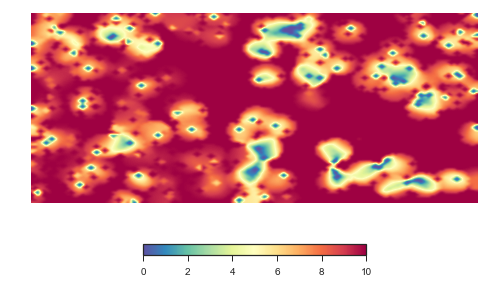
\includegraphics[width=.3\linewidth]{SOM/SOM_TazaLimpia}}
		\newline
		\subfloat[Dulzor]{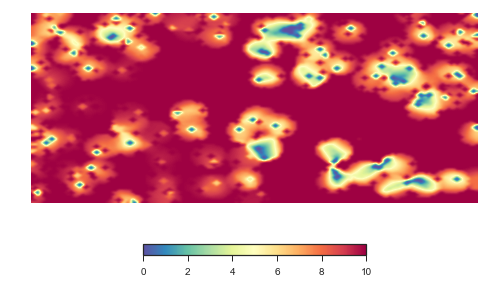
\includegraphics[width=.3\linewidth]{SOM/SOM_Dulzor}}\hfill
		\subfloat[Sabor]{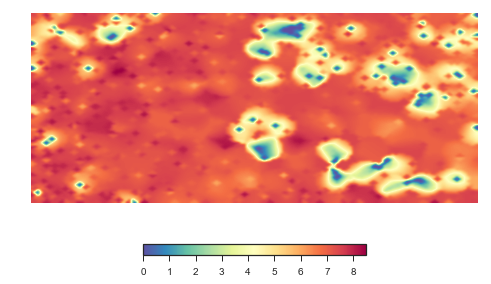
\includegraphics[width=.3\linewidth]{SOM/SOM_Sabor}}\hfill
		\subfloat[Sabor Residual]{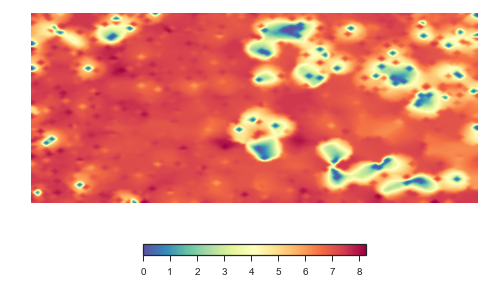
\includegraphics[width=.3\linewidth]{SOM/SOM_SaborResidual}}
		\newline
		\centering
		\subfloat[Puntaje Catador]{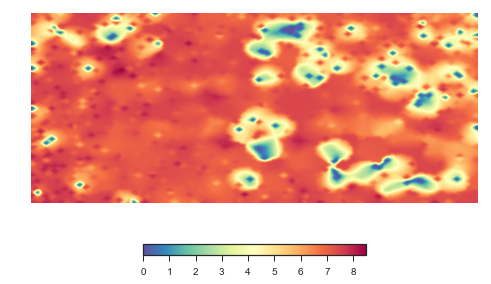
\includegraphics[width=.3\linewidth]{SOM/SOM_PuntajeCatador}}\hfill
		\subfloat[Puntaje Total]{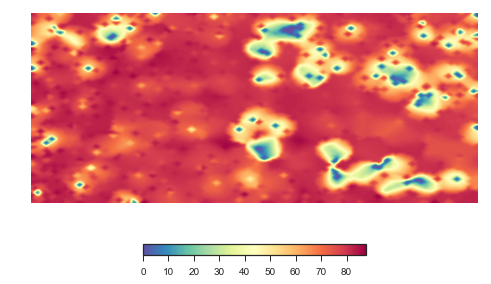
\includegraphics[width=.3\linewidth]{SOM/SOM_PuntajeTotal}}
\end{figure}




\begin{figure}[H]
	\caption{Précipitations}
	\centering
	\subfloat[Prec1]{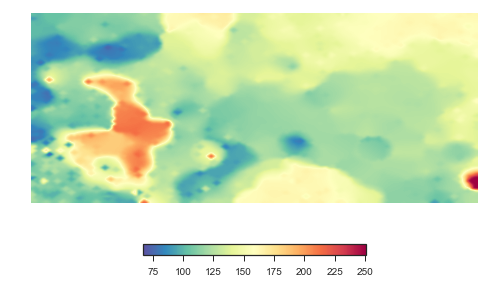
\includegraphics[width=.3\linewidth]{SOM/SOM_Prec1}}\hfill
	\subfloat[Prec2]{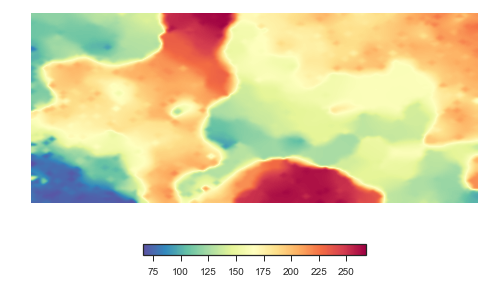
\includegraphics[width=.3\linewidth]{SOM/SOM_Prec2}}\hfill
	\subfloat[Prec3]{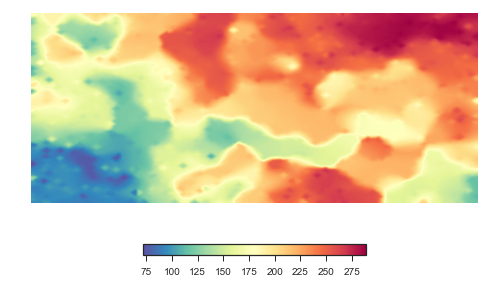
\includegraphics[width=.3\linewidth]{SOM/SOM_Prec3}}\hfill
	\newline
	\subfloat[Prec4]{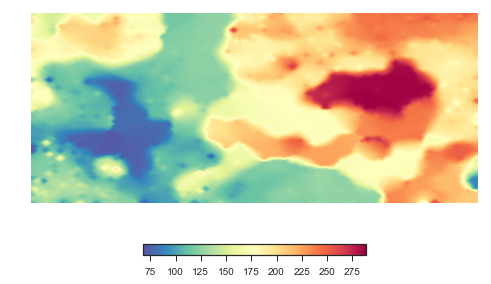
\includegraphics[width=.3\linewidth]{SOM/SOM_Prec4}}\hfill
	\subfloat[Prec5]{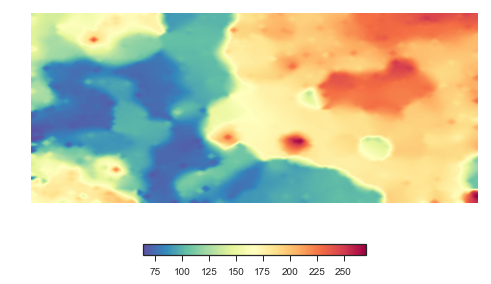
\includegraphics[width=.3\linewidth]{SOM/SOM_Prec5}}\hfill
	\subfloat[Prec6]{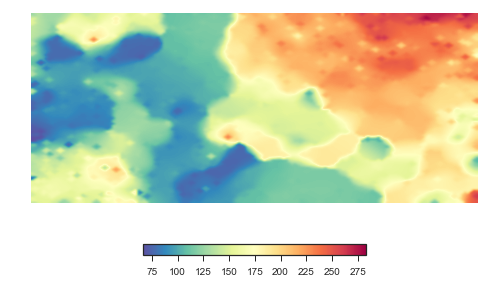
\includegraphics[width=.3\linewidth]{SOM/SOM_Prec6}}\hfill
	\newline
	\subfloat[Prec7]{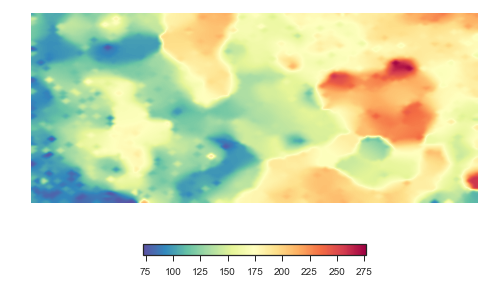
\includegraphics[width=.3\linewidth]{SOM/SOM_Prec7}}\hfill
	\subfloat[Prec8]{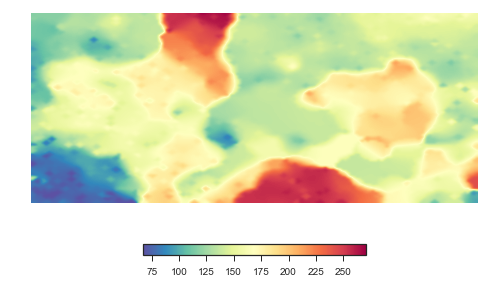
\includegraphics[width=.3\linewidth]{SOM/SOM_Prec8}}\hfill
	\subfloat[Prec9]{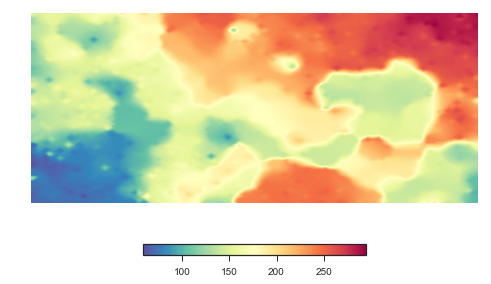
\includegraphics[width=.3\linewidth]{SOM/SOM_Prec9}}\hfill
	\newline
	\centering
	\subfloat[Prec10]{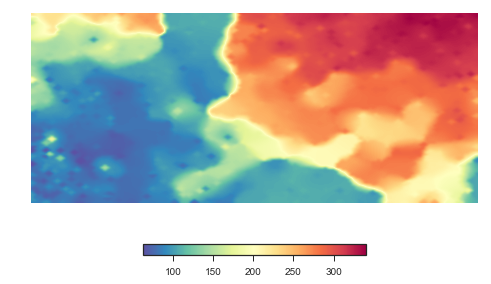
\includegraphics[width=.3\linewidth]{SOM/SOM_Prec10}}
	\subfloat[Average]{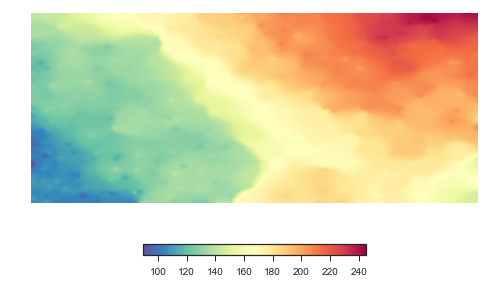
\includegraphics[width=.3\linewidth]{SOM/SOM_PrecTotalAvg}}
\end{figure}



\begin{figure}[H]
	\caption{SOM - Autres données}
	\centering
	\subfloat[Temp. Min. Average]{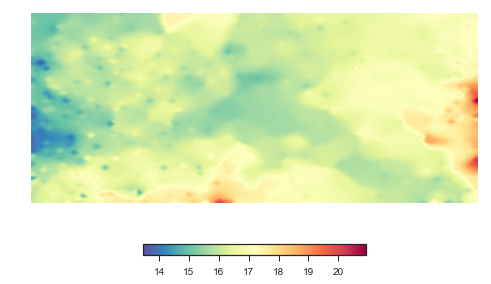
\includegraphics[width=.3\linewidth]{SOM/SOM_TminTotalAvg}}\hfill
	\subfloat[Temp. Max. Average]{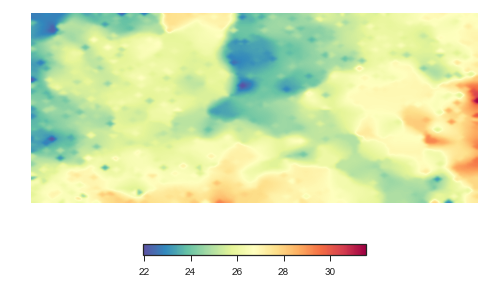
\includegraphics[width=.3\linewidth]{SOM/SOM_TmaxTotalAvg}}\hfill
	\subfloat[Temp. Mean. Average]{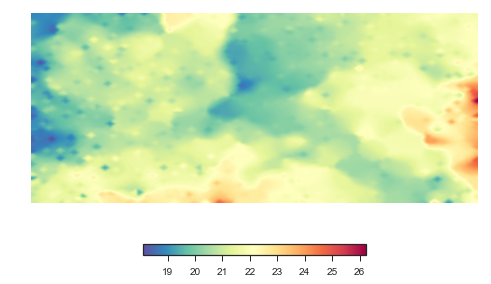
\includegraphics[width=.3\linewidth]{SOM/SOM_TmeanTotalAvg}}\hfill
	\newline
	\subfloat[Dtr Average]{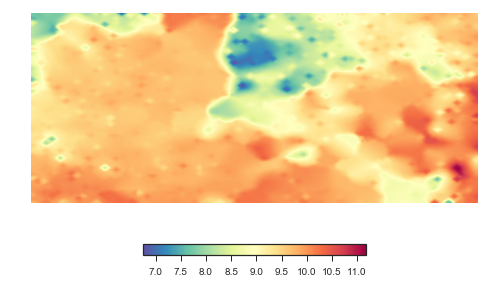
\includegraphics[width=.3\linewidth]{SOM/SOM_DtrTotalAvg}}\hfill
	\subfloat[ASNM]{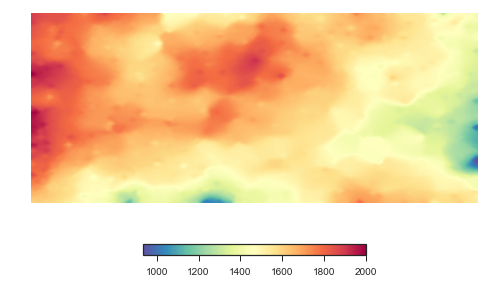
\includegraphics[width=.3\linewidth]{SOM/SOM_ASNM}}\hfill
	\subfloat[Slope]{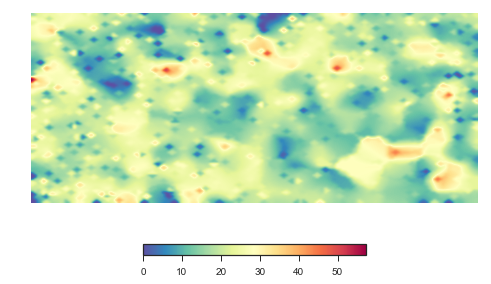
\includegraphics[width=.3\linewidth]{SOM/SOM_Slope}}\hfill
	\newline
	\subfloat[Franco]{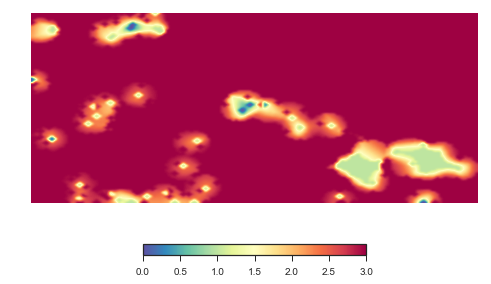
\includegraphics[width=.3\linewidth]{SOM/SOM_Franco}}\hfill
	\subfloat[Arenoso]{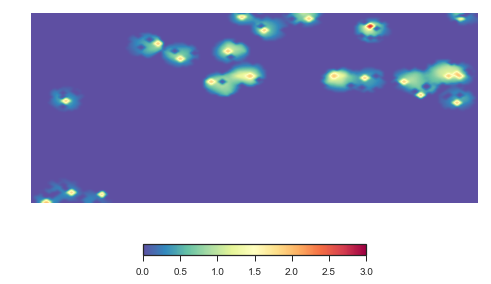
\includegraphics[width=.3\linewidth]{SOM/SOM_Arenoso}}\hfill
	\subfloat[Arcilloso]{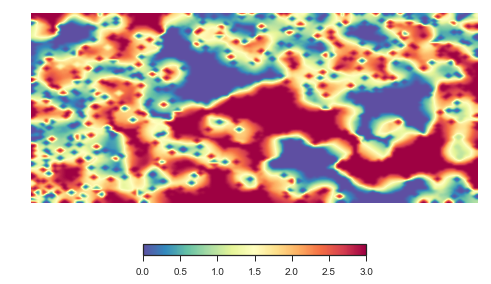
\includegraphics[width=.3\linewidth]{SOM/SOM_Arcilloso}}\hfill
	\newline
	\centering
	\subfloat[Limoso]{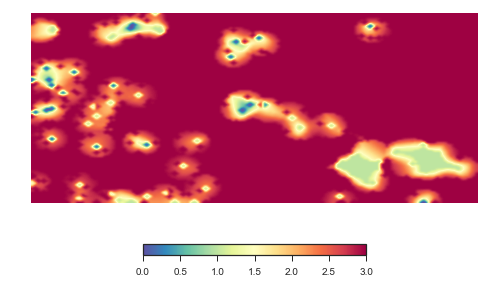
\includegraphics[width=.3\linewidth]{SOM/SOM_Limoso}}\hfill
	\subfloat[Cascajoso]{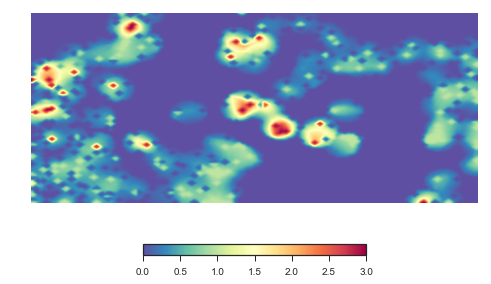
\includegraphics[width=.3\linewidth]{SOM/SOM_Cascajoso}}\hfill
	\subfloat[pH]{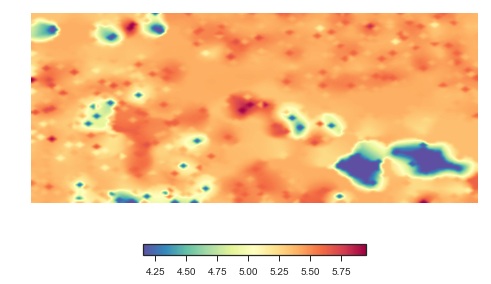
\includegraphics[width=.3\linewidth]{SOM/SOM_pHAvg}}\hfill
	\newline
	\subfloat[Organic]{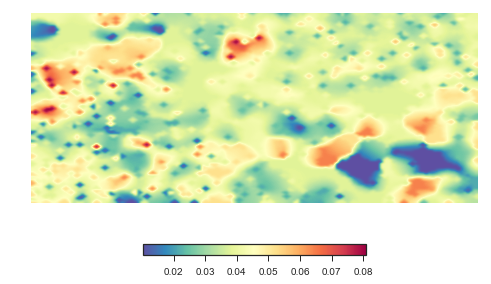
\includegraphics[width=.3\linewidth]{SOM/SOM_OrgAvg}}\hfill
	\subfloat[Orientation]{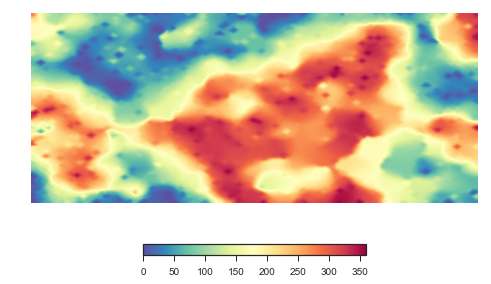
\includegraphics[width=.3\linewidth]{SOM/SOM_OrientationDegrees}}\hfill
	\subfloat[Defectos]{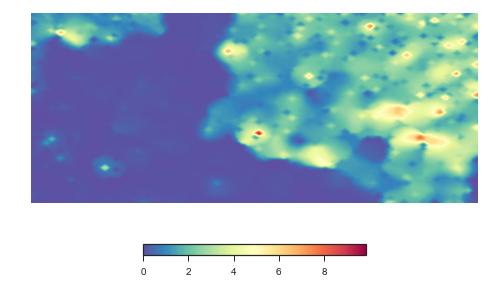
\includegraphics[width=.3\linewidth]{SOM/SOM_DefectosTotales}}
\end{figure}



\begin{figure}[H]
	\caption{\label{SecondSOMASNM}Altitude et défauts lors d'une seconde exécution du réseau de neurones}
	\centering
	\subfloat[ASNM]{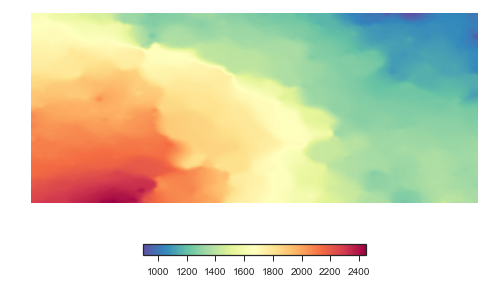
\includegraphics[width=.5\linewidth]{SOM/SOM_ASNM2}}\hfill
	\subfloat[Defectos Totales]{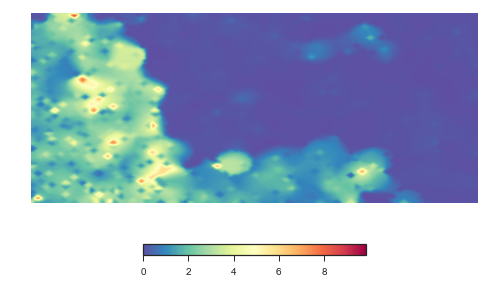
\includegraphics[width=.5\linewidth]{SOM/SOM_DefectosTotales2}}
	\newline

	\centering
	\subfloat[ASNM]{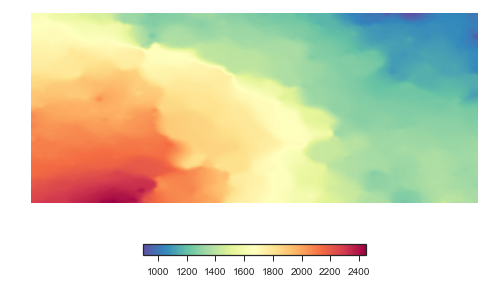
\includegraphics[width=.5\linewidth]{SOM/SOM_ASNM2}}\hfill
	\subfloat[Puntaje Total]{\includegraphics[width=.5\linewidth]{SOM/SOM_PuntajeTotal}}\hfill
	\newline
	\centering 
	\subfloat[Coffee Class Position]{\includegraphics[width=.5\linewidth]{SOM/SOM_Umatrix_Points_Category}}
\end{figure}

On peut observer que les régions avec beaucoup de précipitations sont aussi celles qui ont le plus de cafés avec peu de points. Lors d'une seconde exécution du réseau on a pu observer une relation proche entre les défauts et l'altitude comme montré sur la figure \ref{SecondSOMASNM}. Cette relation n'était pas clairement visible lors de la première exécution. Le fait est déjà connu que le café qui pousse en altitude est de meilleure qualité. On observe sur la figure \ref{AltPts} que la zone en bas à gauche, là où l'altitude est la plus haute, correspond à une zone possédant peu de cafés ayant eu le score 0. 

\newpage
\subsection{Perceptron Multi-couches}
%TODO sur R, sélection de variables avec un MLP, importance des variables 
%TODO tester avec le dataset complet etle dataset compact une fois complété
Waiting for server time



\section{Prédiction}
%Il a été possible ou non de faire de la prédiction, confusion matrix etc
%ce que les méthodes comme random forest ont donné
Le but de cette section est d'analyser la possibilité de prédiction de la qualité des cafés à l'aide des données climatiques et de qualité de sols à disposition. Lorsque l'on parle de la qualité des cafés, on inclue autant les défauts physiques que les résultats de dégustation. 

%TODO faire pour régression et classification -> specialty ou pas -> a ajouter au dataset


\subsection{Random Forest}
% analyser des variables séparément. Possibilité de prédir les défauts vs le "gout", les défauts spéarément - les gouts séparément etc 



\chapter{Analyse des résultats}


%Analyse globale des résultats, discussion sur les résultats 
%Données manquantes

%Exemple: on sait que la fermentation du grain dans sa pulpe impacte sur la chimie de la graine et peut rendre le café plus ou moins acide -> pas de données sur la fermentation (temps, méthode etc) idem pour le séchage, le stockage, la récolte etc
